\chapter{Elektronika}

\section{Součástky}
V této kapitole jsou shrnuty a popsány veškeré elektronické součástky, které jsem v realizování maturitní práce použila.

\subsection{Schematický diagram obvodu}

\begin{figure}[htbp]
	\centering
	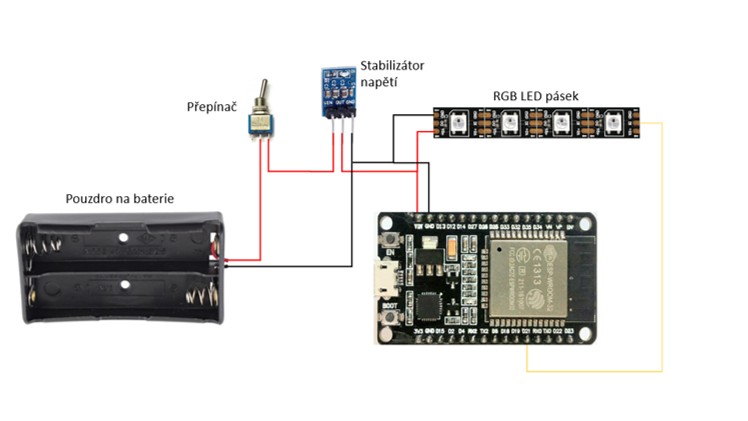
\includegraphics[width=1\textwidth]{img/01 uvod/RGB Schema.png}
	\caption{Zapojení obvodu}
	%	\label{fig:install-sdk-3}
\end{figure}

\subsection{ESP32-DevkitC}
\href{https://www.espressif.com/sites/default/files/documentation/esp32_datasheet_en.pdf}{ESP32-DevKitC} je výkonný programovatelný mikročip s WiFi a Bluetooth modulem, vyvinutý společností \href{https://www.espressif.com}{Espressif}. Je kompatibilní s \href{https://www.arduino.cc}{Arduinem}, se kterým se často využívá v domácích hobby projektech. WiFi a Bluetooth modul dovoluje uživateli se na ESP32-DevKitC připojit pomocí jakéhokoliv dálkového ovladače, nebo mobilního telefonu a se zařízením manipulovat.
Součástí ESP32-DevKitC desky je také micro-USB konektor, který dovoluje jak jednoduché nahrávání programu, tak jednoduché napájení. Pro další manipulaci a využití se po obou stranách desky nachází vstupní a výstupní programovatelné piny, díky kterým lze k ESP32-DevKitC připojit periferní zařízení, nebo zdroj napájení.

\begin{figure}[htbp]
	\centering
	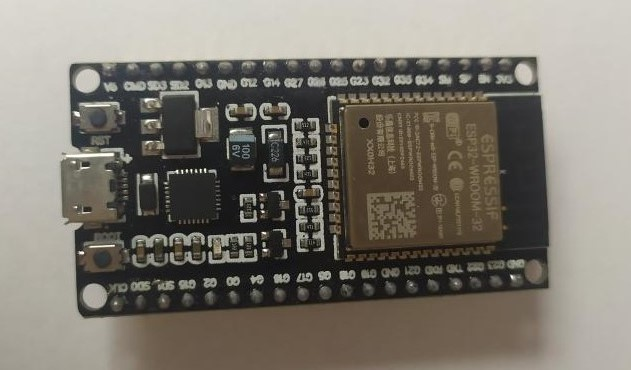
\includegraphics[width=0.5\textwidth]{img/02 ele/ESPDevKit3.jpg}
	\caption{ESP32-DevKitC v4}
	%	\label{fig:install-sdk-3}
\end{figure}

Při realizaci maturitní práce byly použity dvě verze desek: novější verze ESP32-DevKitC v4 a stejně výkonnou, ale vývojově o malinko starší verze ESP32-DevKitC v1. Rozměry obou desek jsou 55mm x 30 mm a liší se pouze pozicí a označením vstupních a výstupních pinů. Jinak je práce a manipulace s nimi stejná. 

\subsection{LED pásek WS2812}

Jedná se o programovatelný ohebný LED pásek, který se z důvodu nízké spotřeby a estetického vzhledu často využívá jako páskové osvětlení do interiérů a exteriérů. Pásek se skládá z řady LED typu \href{https://www.arduino.cc}{WS2812}, které se pomocí kontroléru ve WS diodách dají jednoduše programovat. 

\begin{figure}[htbp]
	\centering
	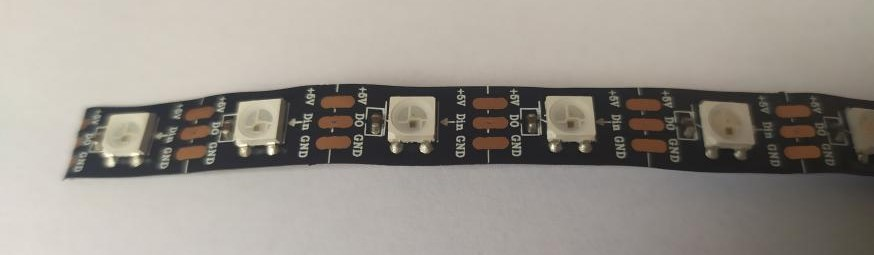
\includegraphics[width=0.5\textwidth]{img/02 ele/OhebnyLedPasek2.jpg}
	%<<<<<<< Updated upstream
	\caption{Pásek WS2812}
	%=======
	%	\caption{Pásek ws2812}
	%>>>>>>> Stashed changes
	%	\label{fig:install-sdk-3}
\end{figure}

Tento pásek se také často využívá jako výstupní modul pro Arduino. Lze ho sehnat v každém obchodě s elektronikou a elektrotechnickými součástkami, často pod marketingovým označením Neopixel. 

\subsection{DC Regulátor napětí 5.5V}

% DollaTek 5.5V DC Voltage Regulator Step Down
Regulátor v obvodu slouží pro sražení vysokého napětí na napětí požadované. Tento \href{https://www.amazon.co.uk/DollaTek-AMS1117-5-5V-Voltage-Regulator-4-75V-12V/dp/B07PPKR4HW/ref=sr_1_21?keywords=step+down+7.4v+to+5v&qid=1639337812&sr=8-21}{DC Regulátor napětí} sráží 5.8V až 12V na napětí 5V. Sama deska ESP32-DevKitC obsahuje vlastní stabilizátor, který sráží napětí z 5V na 3.3V. Jmenovité napětí LED pásku je 5V. Pokud by tedy bylo do obvodu puštěno vyšší napětí, mohlo by dojít jak ke zničení LED pásku, tak desky ESP32-DevKitC.



    \begin{figure}[htbp]
	\centering
	\begin{minipage}[b]{0.5\textwidth}
		\centering
		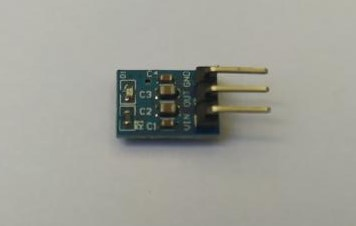
\includegraphics[width=0.75\textwidth]{img/02 ele/Stepdown front.jpg}
		\caption{Stabilizátor zepředu}
		%		\label{fig:gear-sketch1}
	\end{minipage}
	\qquad
	\begin{minipage}[b]{0.4\textwidth}
		\centering
		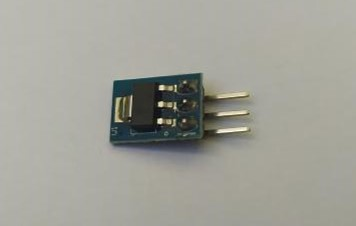
\includegraphics[width=1\textwidth]{img/02 ele/Stepdown back.jpg}
		\caption{Stabilizátor zezadu}
		%		\label{fig:gear-sketch2}
	\end{minipage}
\end{figure}


\section{Možnosti Napájení}

Důležitou součástí obvodu je také napájení, které by mělo mít dostatečně vysoké napětí, aby mohlo napájet obvod. Napájecí napětí obvodu muselo být minimálně 5V. Napadly mě 3 možnosti řešení napájení ESP32-DevKitC a LED pásku.


\subsection{4x AAA baterie 4.8V}

Prvním nápadem bylo využít 4 tužkové AAA baterie s napájecím napětím1.2V, zapojené do série tak, aby jejich výsledné napětí byla 4.8V. Tato možnost se jevila velmi výhodně, protože vzhledem k nízkému napětí nebyl potřeba v obvodu regulátor napětí, a sehnat AAA tužkové baterie je velmi jednoduché. Nevýhodou ale bylo, že by držák na 4 AAA tužkové baterie zabíral v základně hodně místa.
\newpage
Později se ale ukázalo, že není možné využít této možnosti, protože jmenovité napětí LED pásku bylo přesně 5.0V, a i přesto, že ESP32-DevKitC fungoval bezchybně i na 4.8V, LED pásek neměl dostatečně vysoké napětí, aby fungoval. Proto bylo potřeba zvážit jinou alternativu.


\subsection{Napájení Powerbankou}

Další možností bylo využít konektoru, který byl součástí desky  ESP32-DevKitC a přes něj desku napájet Powerbankou.

Výhoda tohoto napájení je, že v obvodu by nebyl potřeba stabilizátor. ESP32-DevKitC je schopno si samo, pomocí svého regulátoru, srážet převyšující napětí a napájet LED pásek pouze na 5V. Při realizaci této možnosti by nebylo potřeba řešit ani baterky, ani regulátor a celkově by se tato možnost vyplatila jako rychlé řešení problému. 

Co se týče umístění powerbanky. Byli zde opět dvě možnosti: %Nenapadlo mě jak jinak to formulovat
První možnost byla sehnat dostatečně malou powerbanku, aby se dala zabudovat do základny společně se zbytkem obvodu. 
%todo Je vážně správné slovo externí? 

Další možností bylo používat Powerbanku, jako externí zdroj, kdykoliv by bylo potřeba světla napájet. Oproti minulé možnosti by mohla mít powerbanku jakoukoliv velikost a tvar a kdyby bylo potřeba, mohla by být nahrazena napájením z počítače nebo jakýkoliv kabelem.  

Stejně tak by nebyl problém s opakovatelným nabíjením Powerbanky.  V případě, že by Powerbanka byla zabudovaná vevnitř, stačilo by jí vytáhnout a znovu přes USB kabel nabít. 
V případě že by Powerbanka sloužila jako externí zdroj, bylo by její znovu-nabíjení ještě jednodušší.
%(kdyby se powerbanka zabudovala dovnitř, základna by byla o mnoho větší než výsledná žárovka a kazilo by to estetický dojem, Dále jsem chtěla, aby byla světla autonomní, aby stačilo pouze zapnout tlačítko. Nelíbila se mi představa, že ze světla bude vést kabel až k powerbance.)


\subsection{Li-ion 18650}

Jako nejvhodnější možnost se mi ale jevilo využití dvou sériově zapojených Li-ion baterií 18650 o napětí 3.6V (dohromady7.2V), jejichž napětí by se muselo srazit regulátorem napětí, ale zajišťovali dostatečný přísun napětí jak pro ESP tak pro LED.  Rozměry baterií v držáku byly 75mm x 42 mm x 20 mm.  Takže Baterie byli dostatečně malé, aby se mohli uložit do základny se zbytkem obvodu.


\begin{figure}[htbp]
	\centering
	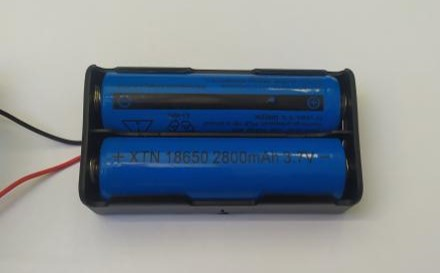
\includegraphics[width=0.45\textwidth]{img/02 ele/Battery_Pack.jpg}
	\caption{Baterky}
	%	\label{fig:install-sdk-3}
\end{figure}

Li-ion baterie lze opakovaně nabíjet na speciální akumulátorové nabíječce, čímž se po delší době může výstupní napětí baterií malinko snížit, což ale v našem případě nevadí, protože přebytek napětí na bateriích je dostatečně vysoký, abychom se nemuseli bát nedostačujícího napětí. 

%Chtěla jsem aby zařízení bylo autonomní


\section{Nabíjení}
Nabíjení by, v případě použití čtyř tužkových baterek AAA, nebylo potřeba vůbec řešit, protože pokud by se baterky vybily, stačilo by jednoduše koupit nové. Stejně tak by nebyl moc velký problém, při použití powerbanky, protože v případě vybití, by stačilo powerbanku jednoduše znovu nabít.

S nabíjením Li-ion baterií to je ale trochu složitější. Ne každý doma vlastní speciální akumulátorovou nabíječku na Li-ion baterie, takže vyřešení nabíjení baterek je oproti dvěma předchozím možnostem napájení o malinko složitější. 
% Tato nabíječka ale není běžnou součástí každé domácnosti. 
Pro vyřešení této problematiky jsem se rozhodla použít tuto součástku:


\subsection{Nabíječka Li-ion článku TP4056 micro-USB}
Jedná se o nabíjecí čip, určený pro nabíjení lithiových akumulátorů, který při připojení k držáku na baterie dovoluje pomocí micro-USB konektoru dané baterie nabíjet. Modul nemá zkratovou ochranu, proto je při práci s ním potřeba opatrnost. Ochrana proti přepětí modulu je do 4.2V, takže pro nás ideální. Dále jsou součástí modulu dvě indikační LED. Červená LED indikuje nabíjení. Modrá LED indukuje kompletní nabití. 
https://www.laskakit.cz/user/related_files/tp4056.pdf
\begin{figure}[htbp]
	\centering
	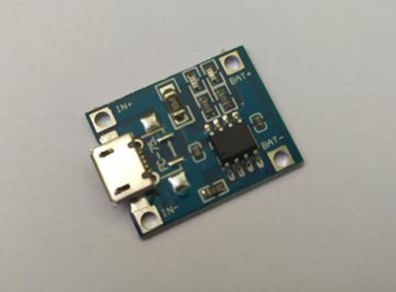
\includegraphics[width=0.3\textwidth]{img/02 ele/Napajeci clanek.jpg}
	\caption{Nabíjecí článek}
	%	\label{fig:install-sdk-3}
\end{figure}

Nabíjení pomocí tohoto článku se dá opět vyřešit dvěma způsoby:


\subsection{Připojit nabíjecí modul přímo do obvodu}
Jedna ze dvou možností, bylo připojit nabíjecí článek přímo do obvodu k bateriím, aby v případě jejich vybití, stačilo sundat vrchní díl základny a pomocí micro-USB konektoru na modulu, obě baterie znovu nabít.
Takhle metoda se zdála lehce nevhodná z důvodu, že by základna po celu dobu nabíjení baterek musela být otevřena. Navíc problematiku jsem začala řešit celkem pozdě, takže ve chvíli, kdy se mi napájecí článek dostal do ruky, měla jsem už obvod spájený/spojený dohromady. Představa, že by se měl ještě upravovat a rozpojovat, aby se do něj vložil nabíjecí modul, nebyla zrovna příjemná.  


\subsection{Vytvořit vlastní nabíječku}
%Vytvořit pomocí nabíjecího článku a držáku na baterky vlastní nabíječku
Druhá možnost se jevila v podstatě přijatelnější. Plánem bylo vzít držák pro dvě baterie a na jeho vývody napájet 2 nabíjecí články. Na každou jednotlivou baterku se napájel článek zvlášť, protože článek neumí napájet baterie v sériovém zapojení.

Tato možnost se jevila jako vhodná a levná alternativa, jak vyřešit nabíjení baterek. 
Problémem zůstává, že vyndávání Li-ion baterií, aby mohli být umístěny do nabíječky, bude celkem obtížné. V tu chvíli se ale tato možnost jevila mnohem jednodušeji, než znovu předělávat celý obvod.
%Bohužel jsem se spletla a zapájela to obráceně. No… Asi to nebylo tak jednoduché jak jsem psala. 

    \begin{figure}[htbp]
	\centering
	\begin{minipage}[b]{0.45\textwidth}
		\centering
		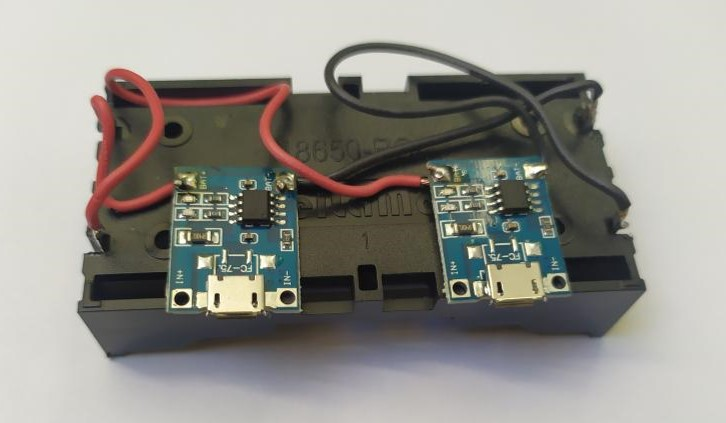
\includegraphics[width=1\textwidth]{img/02 ele/Nabijecka.jpg}
		\caption{Nabíječka zepředu}
		%		\label{fig:gear-sketch1}
	\end{minipage}
	\qquad
	\begin{minipage}[b]{0.45\textwidth}
		\centering
		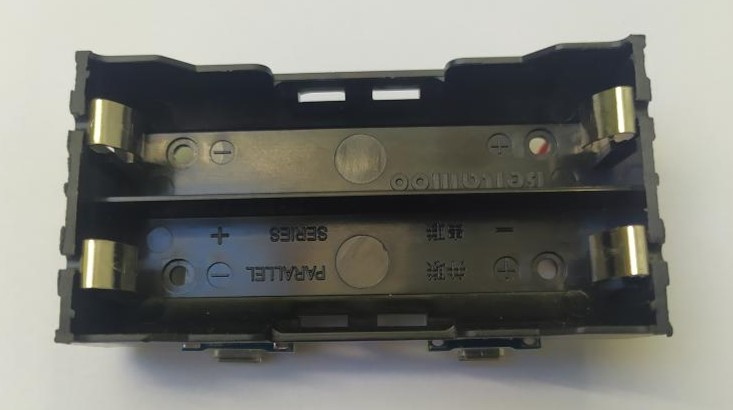
\includegraphics[width=1\textwidth]{img/02 ele/Nabijecka 2.jpg}
		\caption{Nabíječka zezadu}
		%		\label{fig:gear-sketch2}
	\end{minipage}
\end{figure}
\newpage



